In this section, we discuss the performance of \pred\ with respect to the increasing number of tasks for the linear bandit setting. Again note that the number of tasks $\Mpr \gg A \geq n$.
% 
%
Through this experiment, we want to evaluate the performance of \pred\ to exploit the underlying reward correlation when the horizon is small and the number of tasks is changing.
%
Finally, recall that when the horizon is small the weak demonstrator $\pi^w$ does not have sufficient samples for each action. This leads to a poor approximation of the greedy action. 


\textbf{Baselines:} We again implement the same baselines discussed in \Cref{sec:short-horizon}. The baselines are \pred, \predt, \dptg, \ad, \ts, and \linucb. 


\textbf{Outcomes:} We first discuss the main outcomes of our experimental results for increasing the horizon:

\begin{tcolorbox}
\customfinding \pred\ (\gt) fails to exploit the underlying latent structure and reward correlation from in-context data when the number of tasks is small. 
\end{tcolorbox}

% \noindent
% \textbf{(1)} The \pred\ (\gt) fails to exploit the underlying latent structure and reward correlation when the number of tasks is small.

% \textbf{(2)} As the number of tasks increases the \pred\ (\gt) learns the latent structure and the underlying reward correlation.

% \textbf{(3)} The \pred\ (\gt) has lower regret compared to \dptg, \ad\ with increasing number of tasks.




% \begin{figure}[!hbt]
% \centering
% \begin{tabular}{ccc}
% \subfigure[Tasks $\Mtr=5000$]{\hspace*{-1.5em}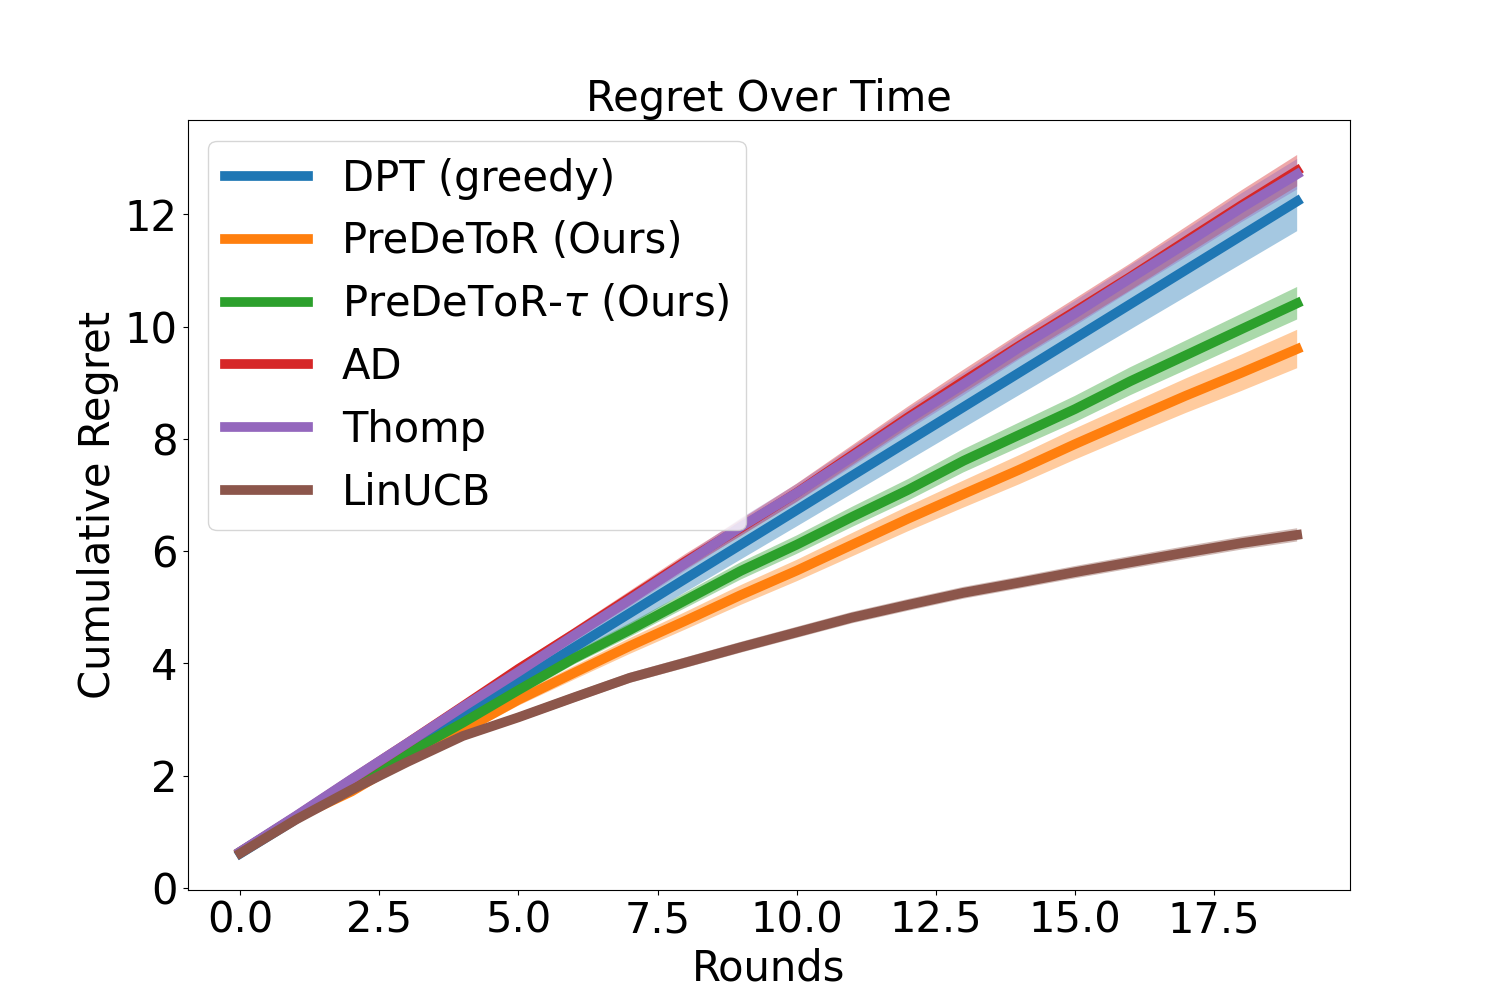
\includegraphics[scale = 0.13]{img/Neurips/inc_env/lin_e5_lr0.00015_do0_embd32_layer4_head4_envs5000_hists1_samples1_var0.3_cov0.0_H20_d40_lind10_seed1_testcov0.0_hor20.pkl.png}\label{fig:env-5}} &
% %%%%%%%%%%
% \hspace*{-1.5em}\subfigure[Tasks $\Mtr=10000$]{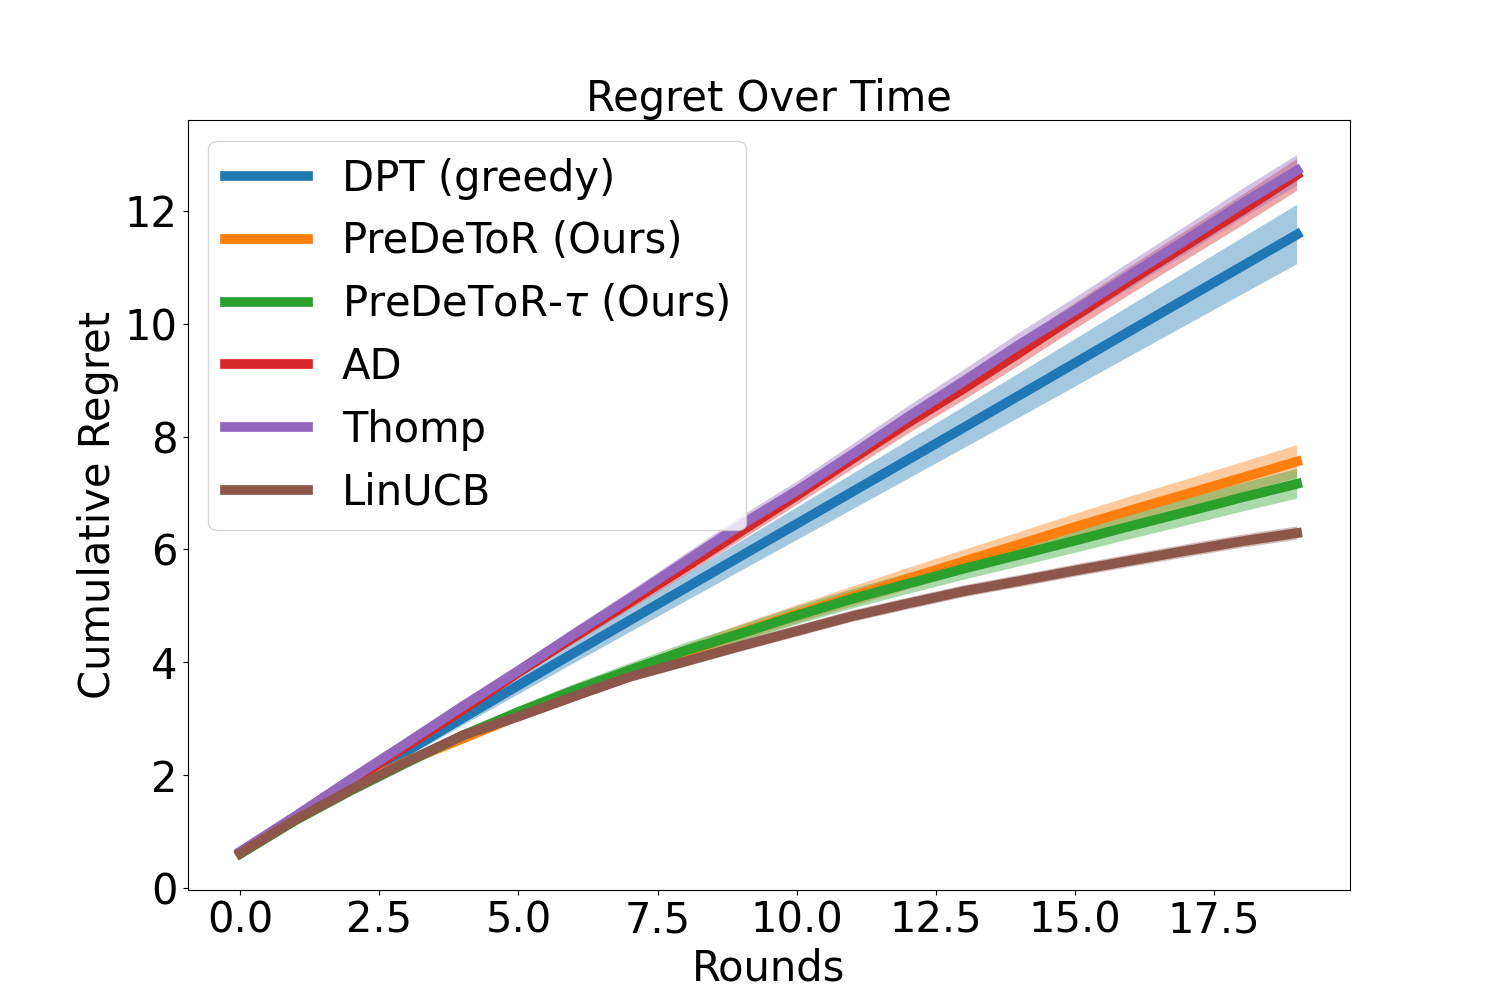
\includegraphics[scale = 0.13]{img/Neurips/inc_env/lin_e10_lr0.00015_do0_embd32_layer4_head4_envs10000_hists1_samples1_var0.3_cov0.0_H20_d40_lind10_seed1_testcov0.0_hor20.pkl.png} \label{fig:env-10}} &
% %%%%%%%%%%%%%%%%%%%%%%%
% \subfigure[Tasks $\Mtr=50000$]{\hspace*{-1.5em}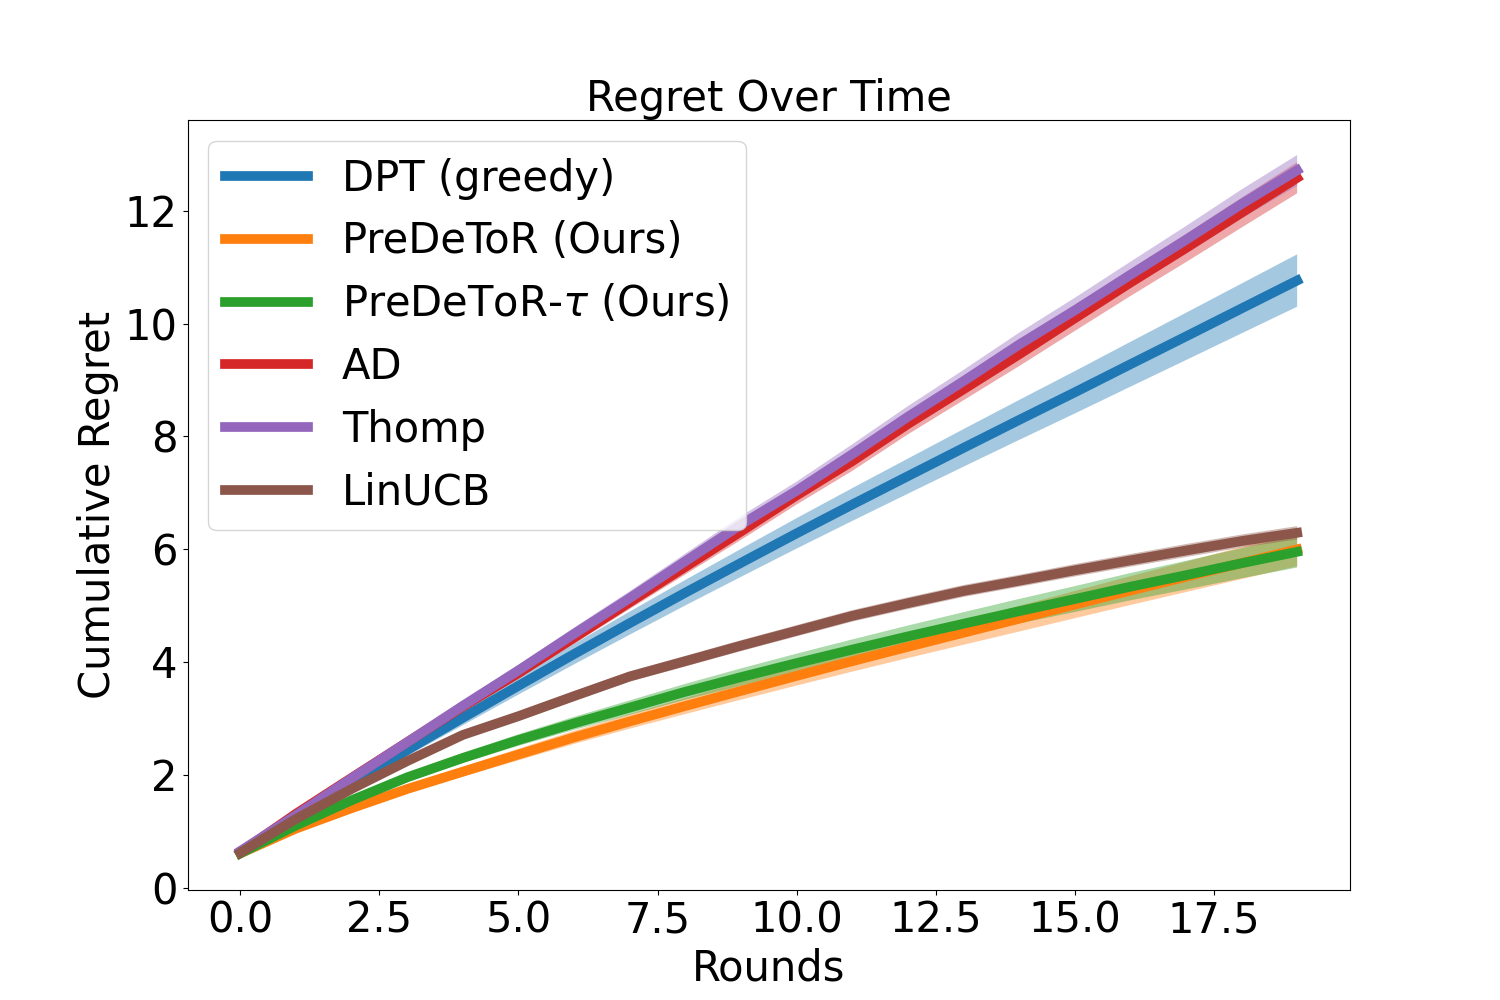
\includegraphics[scale = 0.13]{img/Neurips/inc_env/lin_e100_lr0.00015_do0_embd32_layer4_head4_envs100000_hists1_samples1_var0.3_cov0.0_H20_d40_lind10_seed1_testcov0.0_hor20.pkl.png}\label{fig:env-50}} \\
% %%%%%%%%%%
% %%%%%%%%%%
% %%%%%%%%%%
% \hspace*{-1.5em}\subfigure[Tasks $\Mtr=100000$]{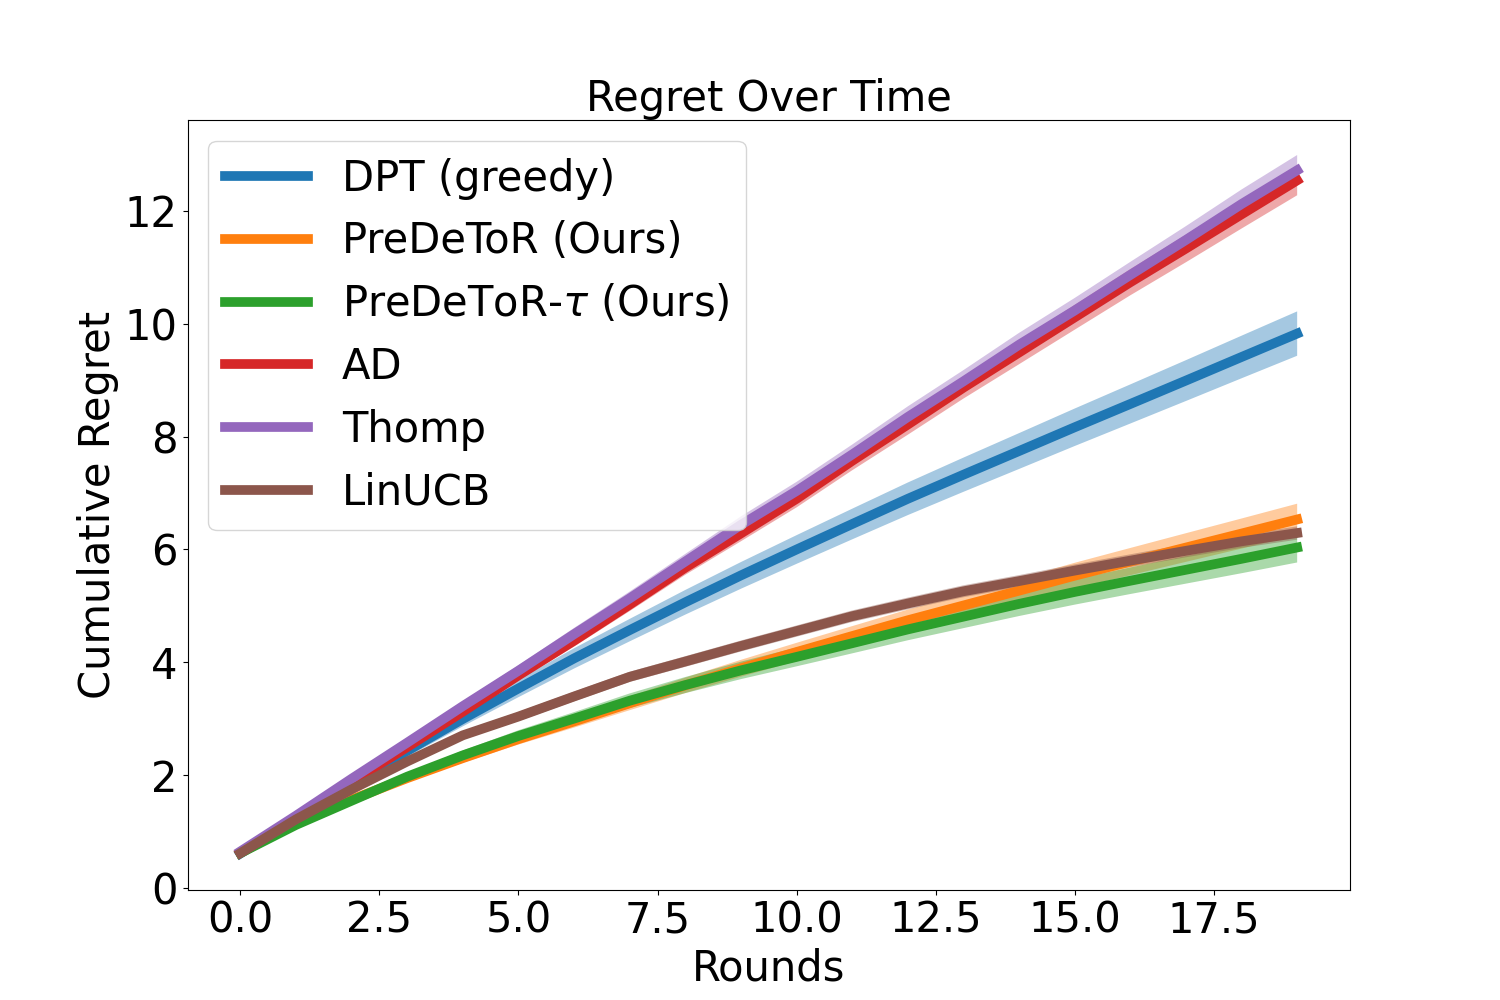
\includegraphics[scale = 0.13]{img/Neurips/inc_env/lin_e150_lr0.00015_do0_embd32_layer4_head4_envs150001_hists1_samples1_var0.3_cov0.0_H20_d40_lind10_seed1_testcov0.0_hor20.pkl.png} \label{fig:env-100}} &
% %%%%%%%%%%%%%%%%%%%%%%%%%%%%%%%
% \hspace*{-1.5em}\subfigure[Tasks $\Mtr=150000$]{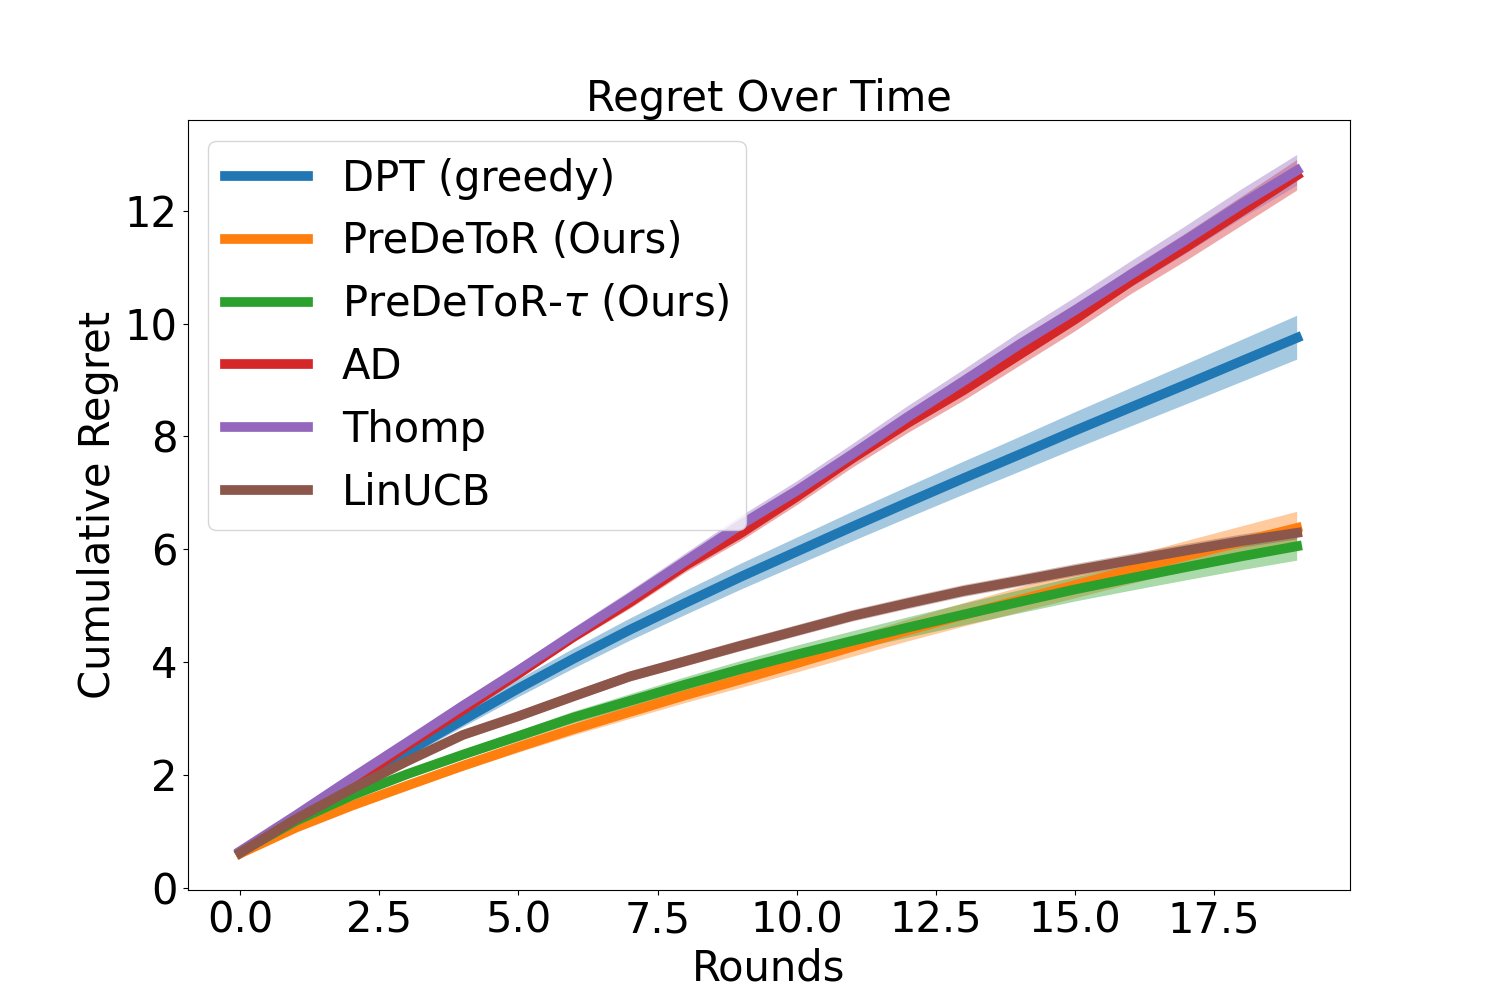
\includegraphics[scale = 0.13]{img/Neurips/inc_env/lin_e200_lr0.00015_do0_embd32_layer4_head4_envs200008_hists1_samples1_var0.3_cov0.0_H20_d40_lind10_seed1_testcov0.0_hor20.pkl.png} \label{fig:env-150}} &
% %%%%%%%%%%%%%%%%%%%%%%%%%%%%%%%%%
% \subfigure[Increasing tasks]{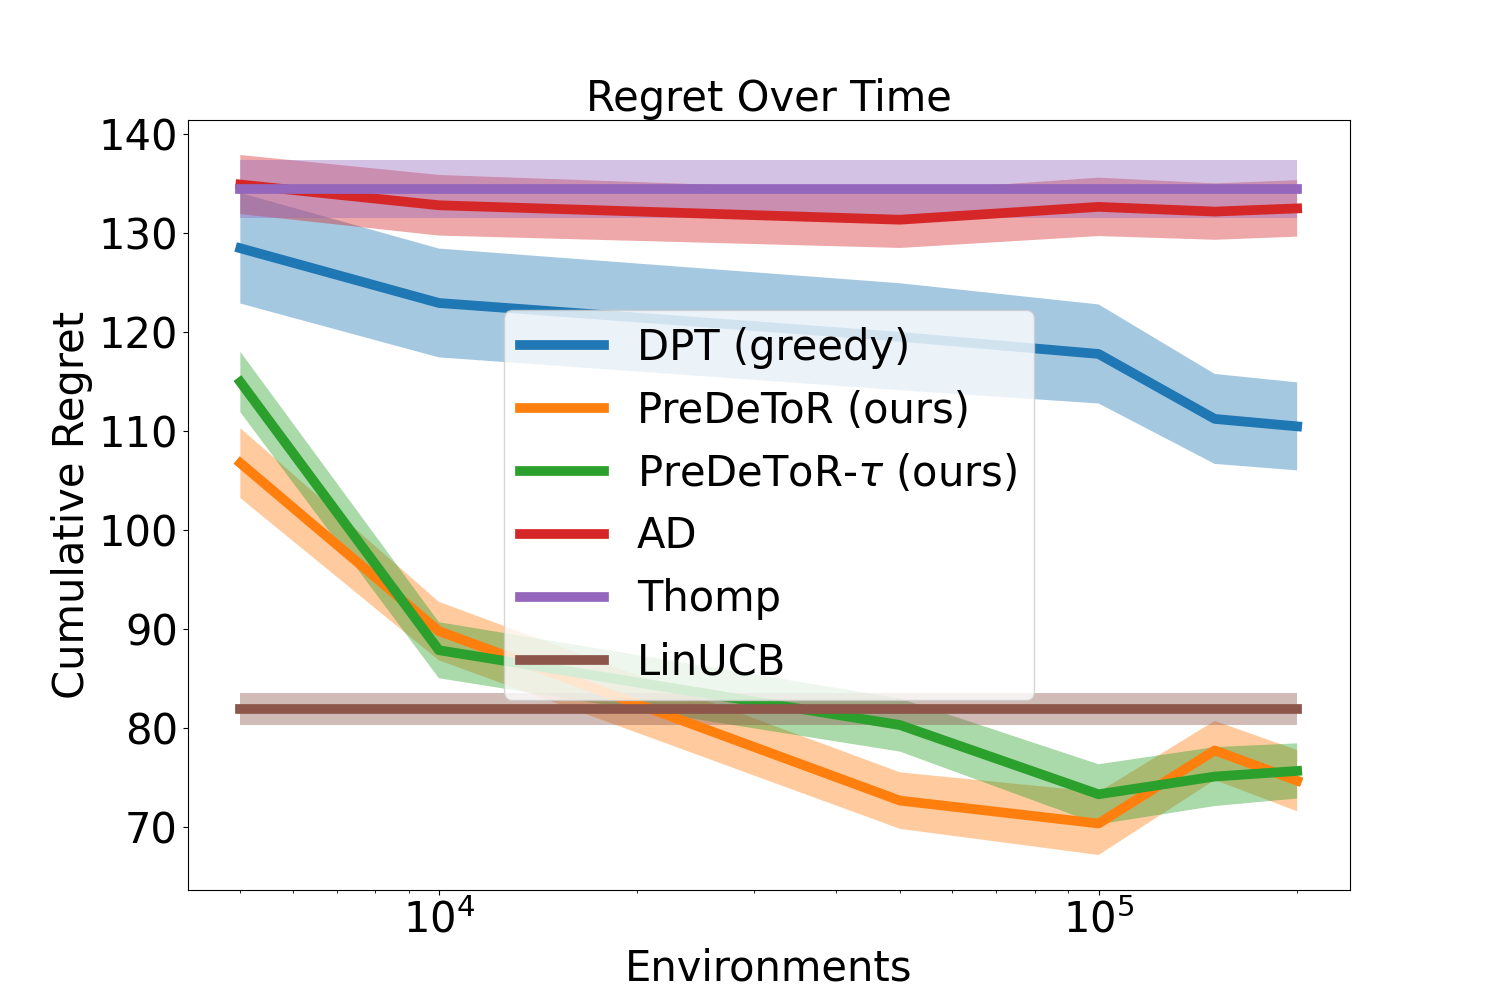
\includegraphics[scale = 0.13]{img/Neurips/inc_env/env_fig.png} \label{fig:env-200}}
% \end{tabular}
% \vspace*{-1em}
% \caption{Experiment with an increasing number of tasks. The y-axis shows the cumulative regret.}
% \label{fig:expt-inc-env}
% \vspace{-0.7em}
% \end{figure}


\begin{figure}[!hbt]
\centering
\begin{subfigure}[b]{0.32\textwidth}
   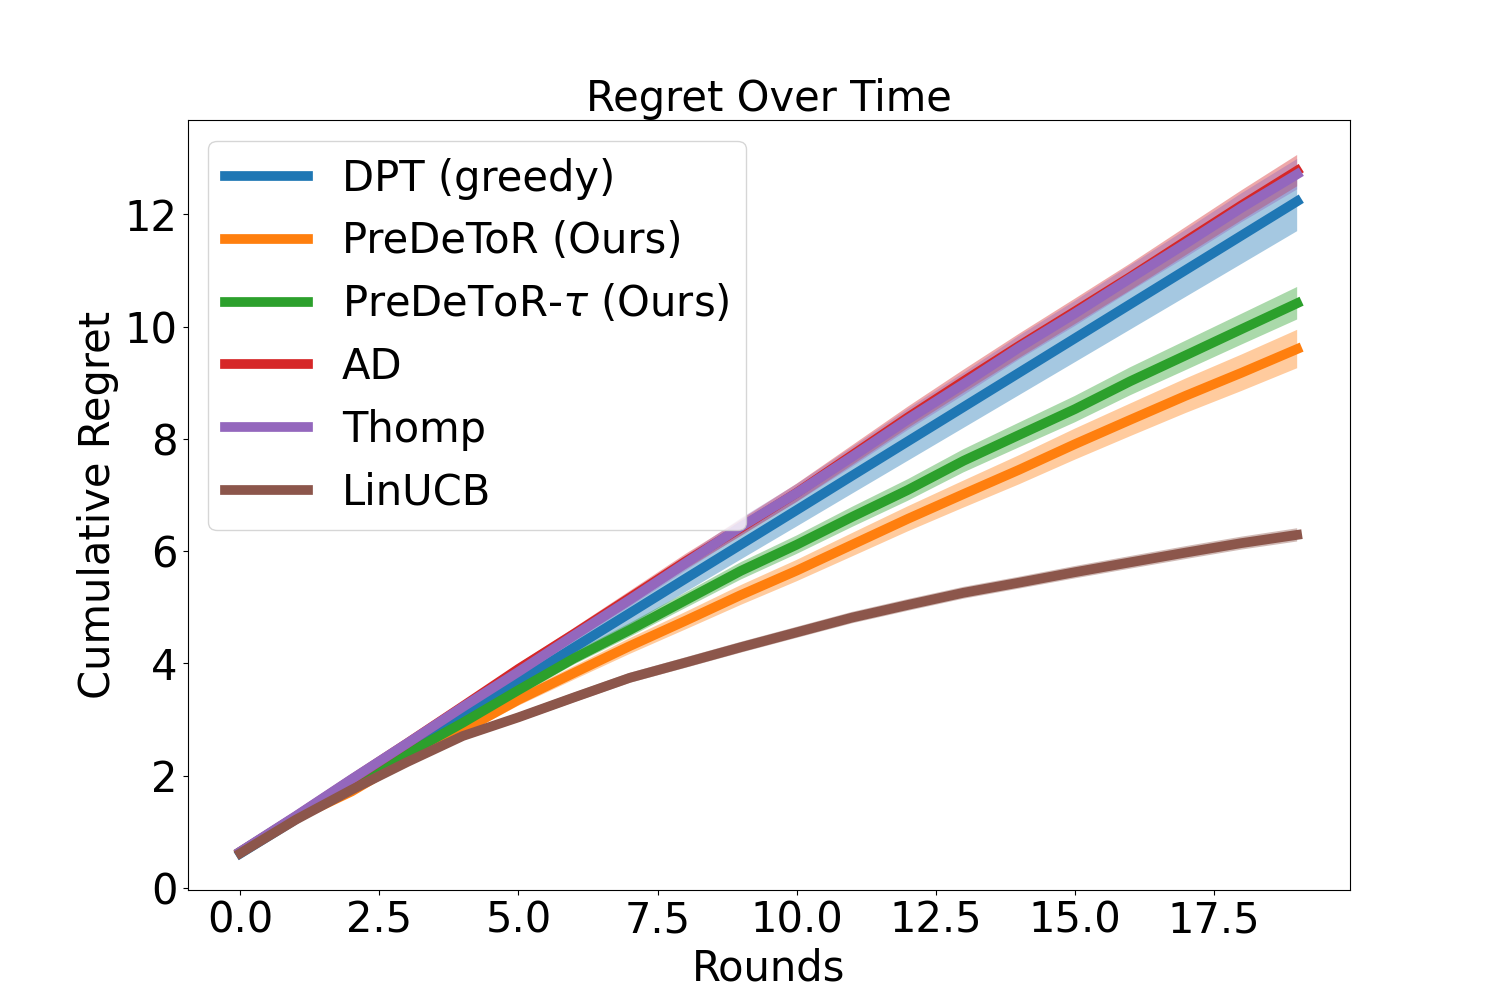
\includegraphics[scale=0.13]{img/Neurips/inc_env/lin_e5_lr0.00015_do0_embd32_layer4_head4_envs5000_hists1_samples1_var0.3_cov0.0_H20_d40_lind10_seed1_testcov0.0_hor20.pkl.png}
   \caption{Tasks $\Mtr=5000$}
   \label{fig:env-5}
\end{subfigure}%
\begin{subfigure}[b]{0.32\textwidth}
   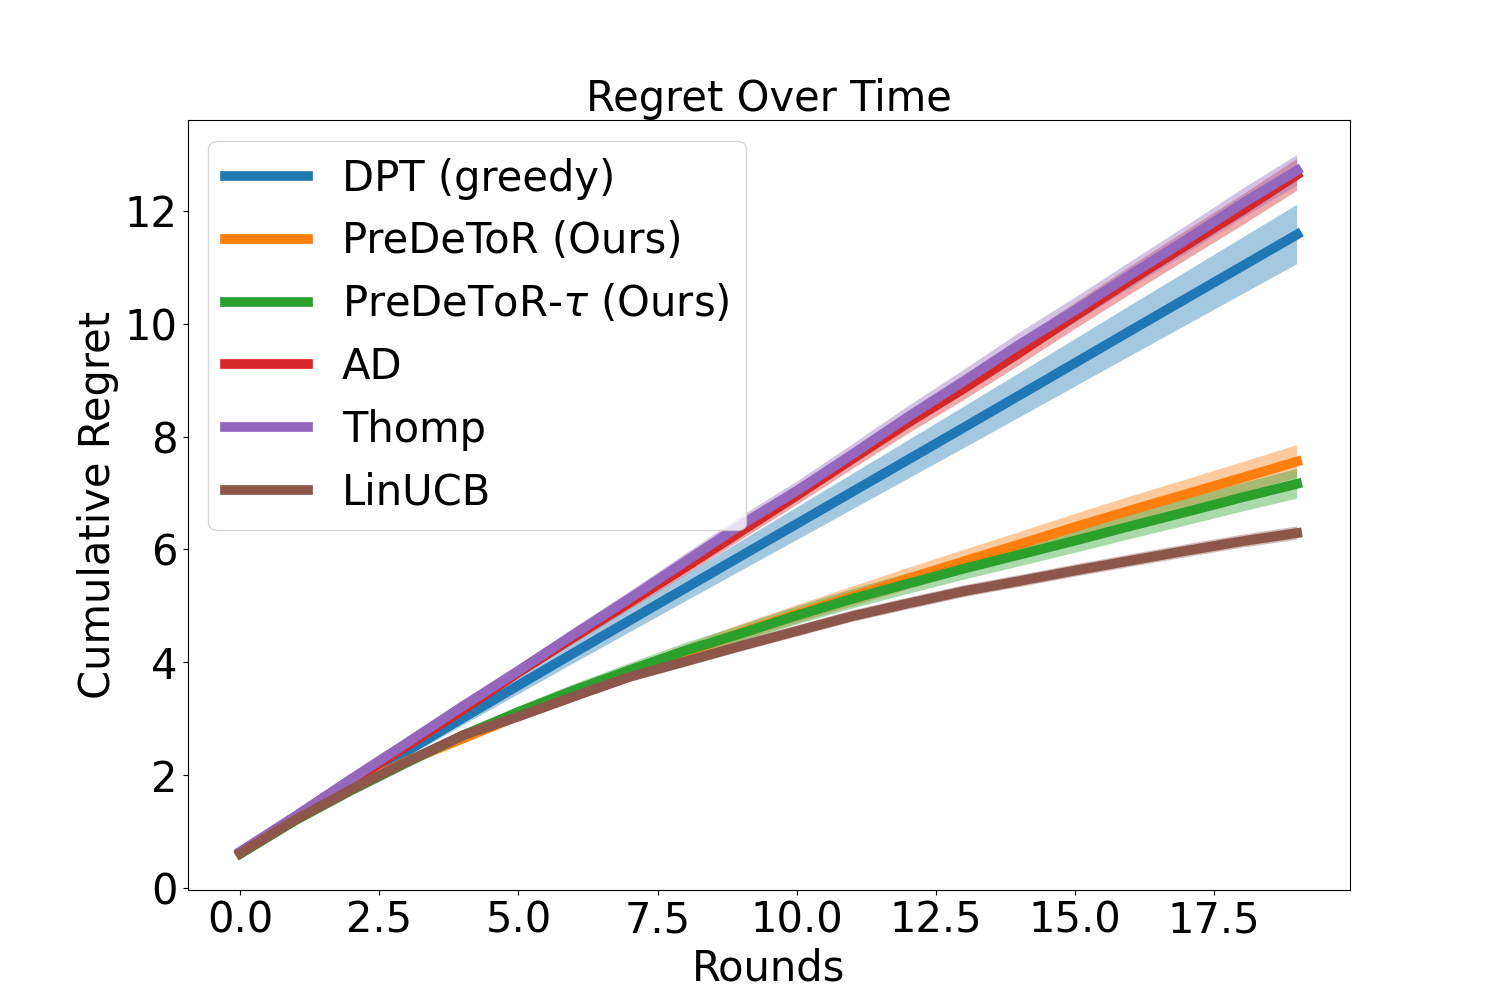
\includegraphics[scale=0.13]{img/Neurips/inc_env/lin_e10_lr0.00015_do0_embd32_layer4_head4_envs10000_hists1_samples1_var0.3_cov0.0_H20_d40_lind10_seed1_testcov0.0_hor20.pkl.png}
   \caption{Tasks $\Mtr=10000$}
   \label{fig:env-10}
\end{subfigure}%
\begin{subfigure}[b]{0.32\textwidth}
   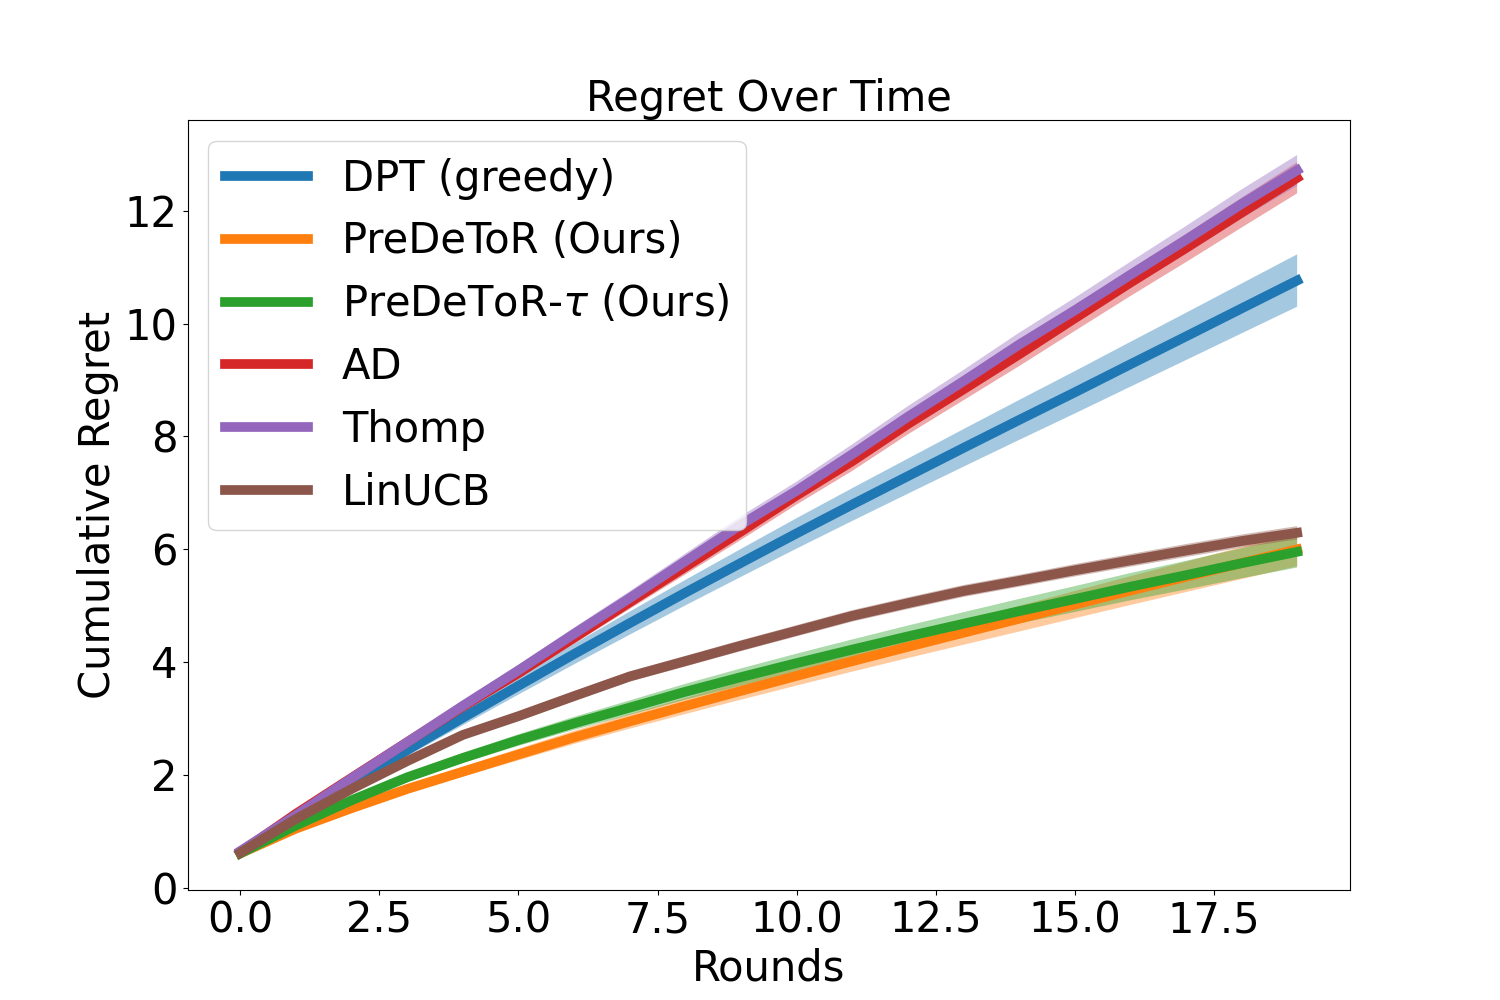
\includegraphics[scale=0.13]{img/Neurips/inc_env/lin_e100_lr0.00015_do0_embd32_layer4_head4_envs100000_hists1_samples1_var0.3_cov0.0_H20_d40_lind10_seed1_testcov0.0_hor20.pkl.png}
   \caption{Tasks $\Mtr=50000$}
   \label{fig:env-50}
\end{subfigure}

\begin{subfigure}[b]{0.32\textwidth}
   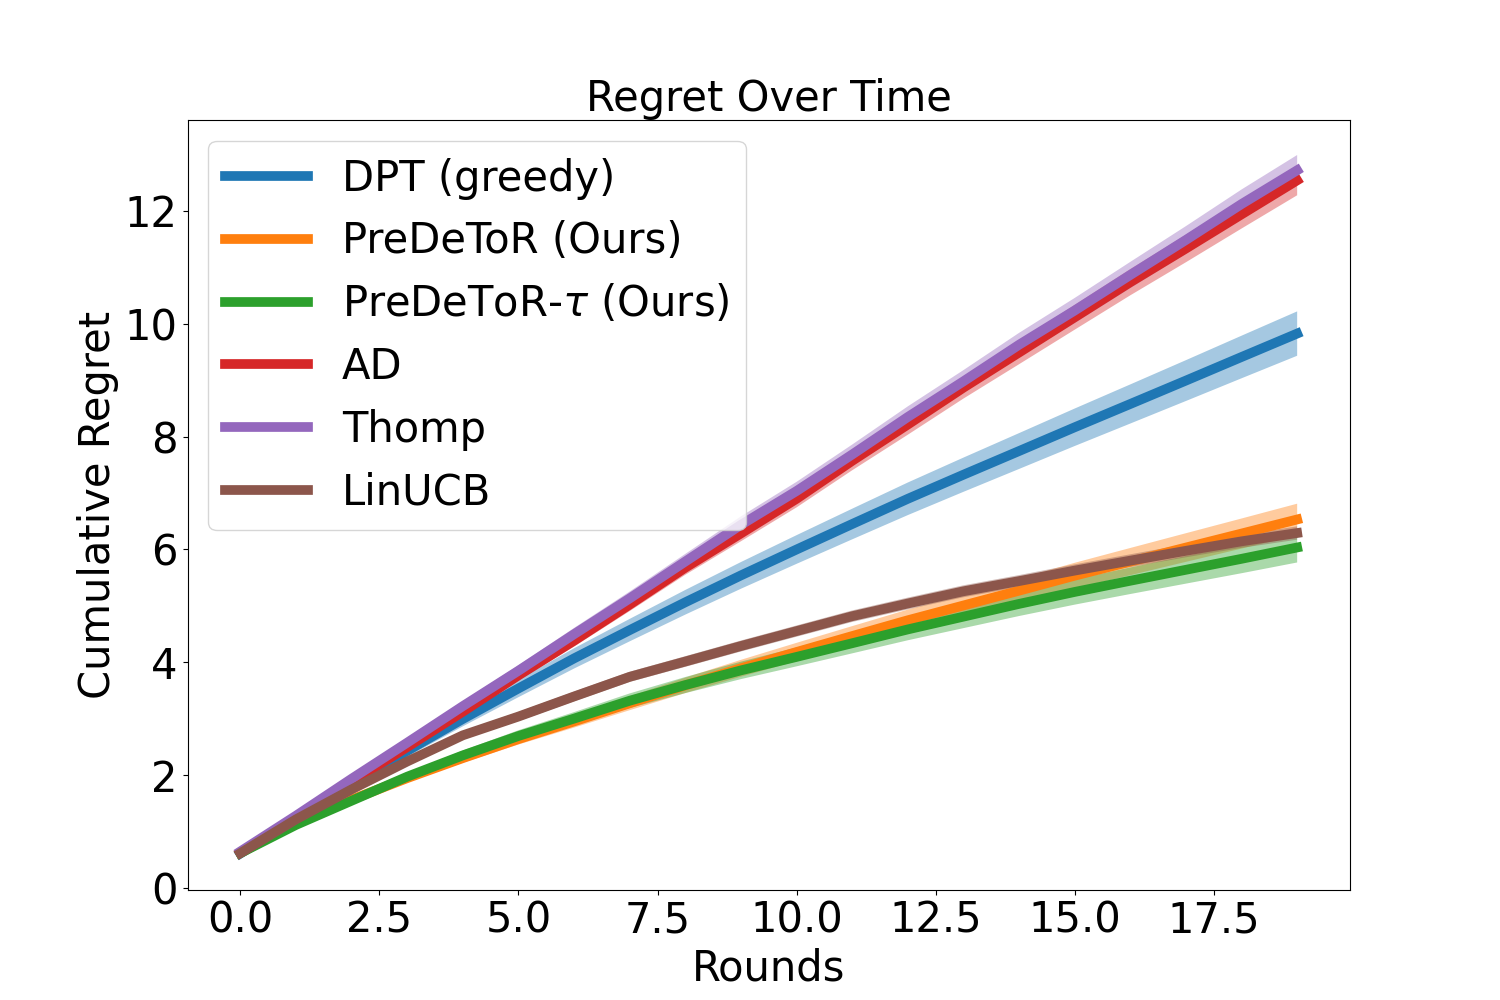
\includegraphics[scale=0.13]{img/Neurips/inc_env/lin_e150_lr0.00015_do0_embd32_layer4_head4_envs150001_hists1_samples1_var0.3_cov0.0_H20_d40_lind10_seed1_testcov0.0_hor20.pkl.png}
   \caption{Tasks $\Mtr=100000$}
   \label{fig:env-100}
\end{subfigure}%
\begin{subfigure}[b]{0.32\textwidth}
   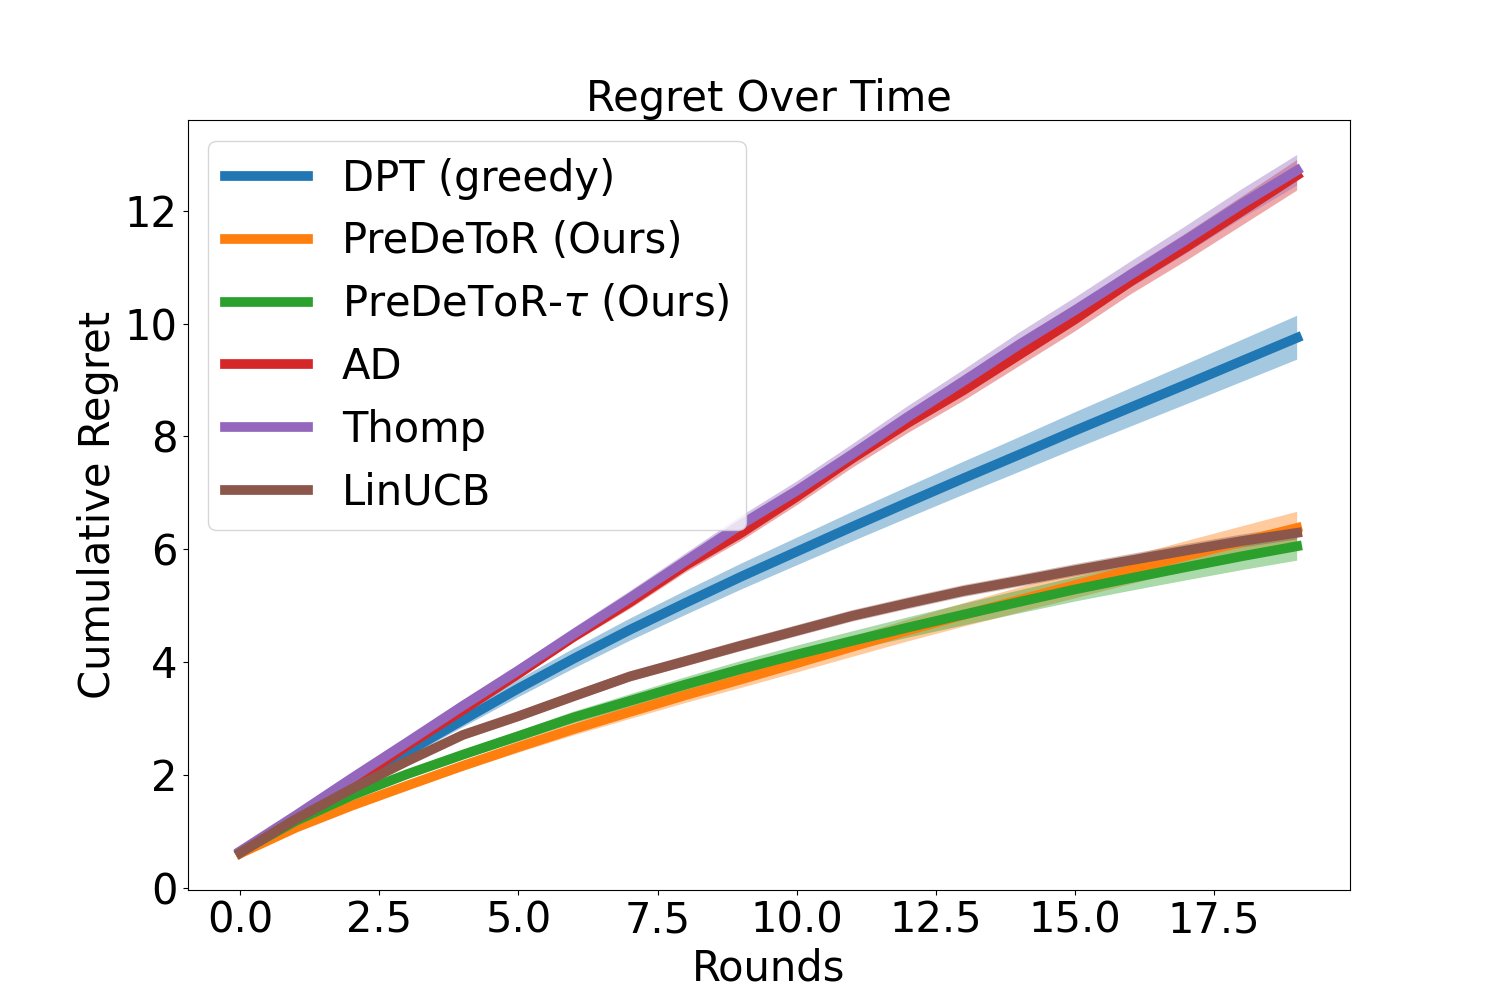
\includegraphics[scale=0.13]{img/Neurips/inc_env/lin_e200_lr0.00015_do0_embd32_layer4_head4_envs200008_hists1_samples1_var0.3_cov0.0_H20_d40_lind10_seed1_testcov0.0_hor20.pkl.png}
   \caption{Tasks $\Mtr=150000$}
   \label{fig:env-150}
\end{subfigure}%
\begin{subfigure}[b]{0.32\textwidth}
   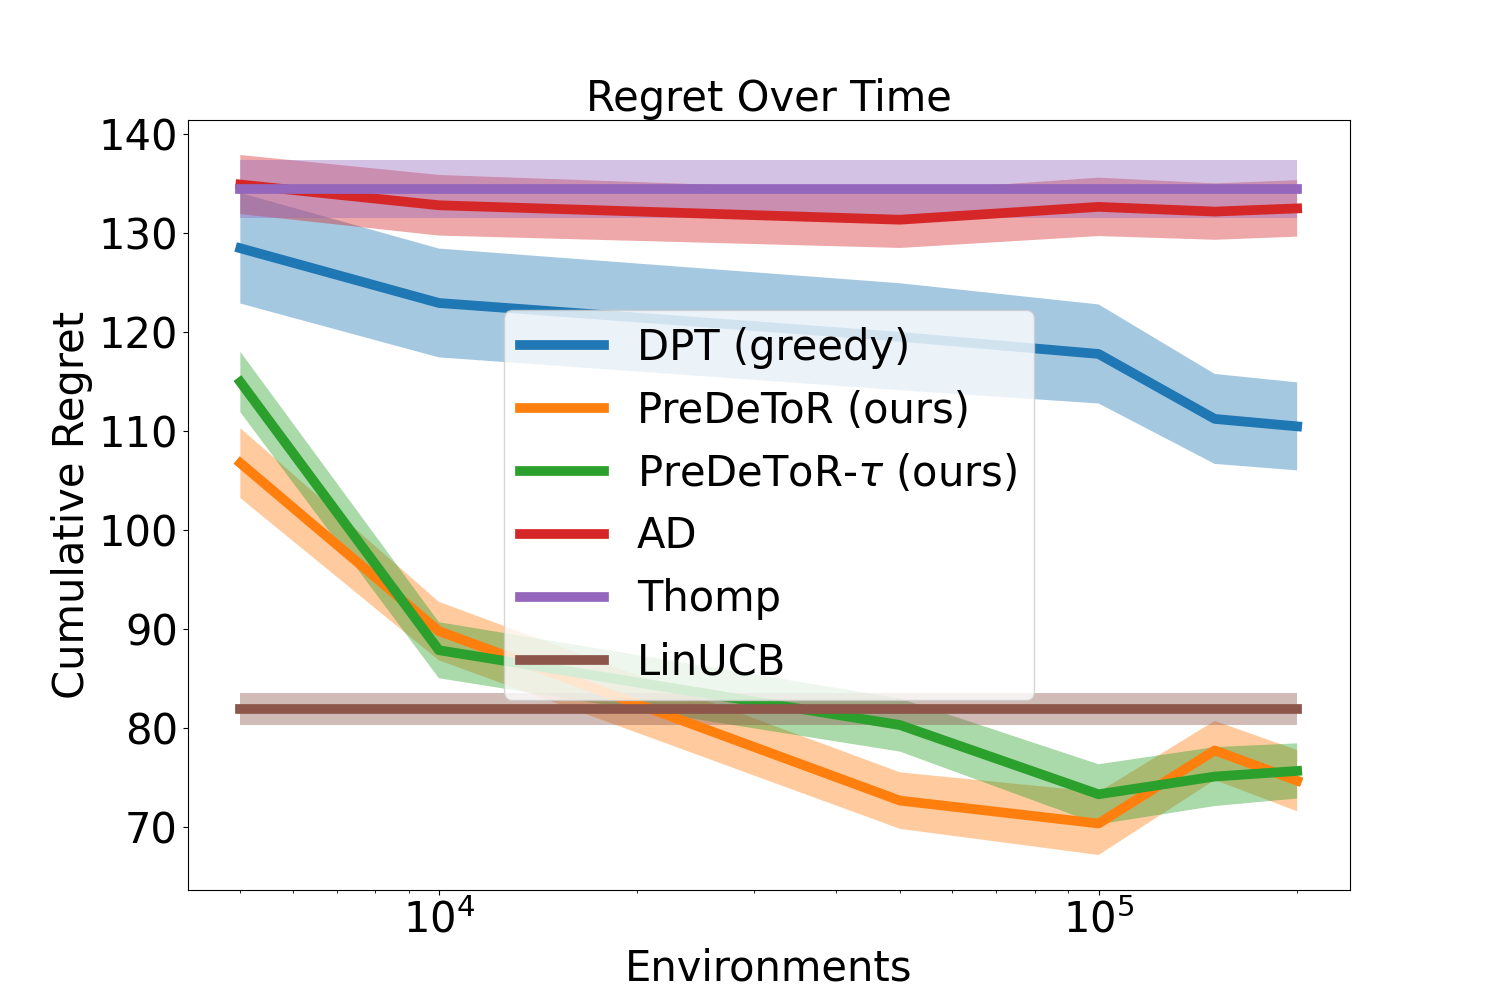
\includegraphics[scale=0.13]{img/Neurips/inc_env/env_fig.png}
   \caption{Increasing tasks}
   \label{fig:env-200}
\end{subfigure}
\vspace*{-1em}
\caption{Experiment with an increasing number of tasks. The y-axis shows the cumulative regret.}
\label{fig:expt-inc-env}
\vspace{-0.7em}
\end{figure}

\textbf{Experimental Result:} We observe these outcomes in \Cref{fig:expt-inc-env}. In \Cref{fig:expt-inc-env} we show the linear bandit setting for horizon $n=20$, $\Mpr  \in \{5000, 10000, 50000, 100000, 150000\}$, $\Mts = 200$, $A=20$, and $d=40$. 
%
%
Again, the demonstrator $\pi^w$ is the \ts\ algorithm. We observe that \pred\ (\gt), \ad\ and \dptg\ suffer more regret than the \linucb\ when the number of tasks is small ($\Mtr\in\{5000, 10000\}$ in \Cref{fig:env-5}, and \ref{fig:env-10}. However in \Cref{fig:env-50}, \ref{fig:env-100}, \ref{fig:env-150}, and \ref{fig:env-200} we show that \pred\ has lower regret than \ts\ and matches \linucb. This shows that \pred\ (\gt) is exploiting the latent linear structure of the underlying tasks for the non-linear setting.
%
%
Moreover, observe that as $\Mtr$ increases the \pred\ has lower cumulative regret than \dptg, \ad. Note that for any task $m$ for the horizon $20$ the \ts\ will be able to sample all the actions at most once. Therefore \dptg\ does not perform as well as \pred.
%
% The training of \ad\ ensures that it does not outperform the demonstrator \ts.
%
Finally, note that the result shows that \pred\ (\gt) is able to exploit the reward correlation across the tasks better as the number of tasks increases.

% Moreover \pred\ matches the performance of \linucb. 
%
%The weak performance of \dptg\ can be attributed to both short horizons and the inability to estimate the optimal action for such a short horizon $H < A$. 
%
%Note that for this small horizon setting the \dptg\ does not have a good estimation of $\widehat{a}_{m,*}$ which results in a poor prediction of optimal action $\widehat{a}_{m,t,*}$. 
% This results in higher regret. 
% Observe from \Cref{fig:head-2}, \ref{fig:head-4}, \ref{fig:head-6}, and \ref{fig:head-8} that \pred\ has lower regret than \ts\ and \linucb\ which also shows that \pred\ is learning the latent linear structure of the underlying tasks for the non-linear setting.
% %
% In \Cref{fig:head-inc} we plot the regret of all the baselines with respect to the increasing attention heads. Again we see that \pred\ regret decreases as we increase the attention heads. This shows that \pred\ training procedure is able to capture the reward correlation better and hence predict the reward of the optimal action more efficiently.